\documentclass{article}

\usepackage{graphicx}
\usepackage{subfigure}
\usepackage[hypcap]{caption}

\title{Experimental Design and Data Analysis: Assignment 2}
\author{Andrew Bedard \& Simone van Gompel(2567525) \\ Group 19}

\begin{document}

  \maketitle

  \section{Exercise 1}
    Exercise 1 stuff...

  \section{Exercise 2}
    I needed to put the light1882 on 1 line, else it can't be imported as a table,
    because it would not have a full last line.
    See Fig:\ref{fig:HistEx2} for the histograms of the two datasets.\\
    The 95\% confidence interval of the mean of Light1879 is 836.7226 - 868.0774\\
    The 95\% confidence interval of the mean of Light1879 is 712.4417 - 799.9931\\
    The 95\% confidence interval of the median of Light1879 is 834.5142 - 865.4858\\
    The 95\% confidence interval of the median of Light1879 is 730.2243 - 817.7757\\

    \begin{figure}
      \subfigure[1879]
      {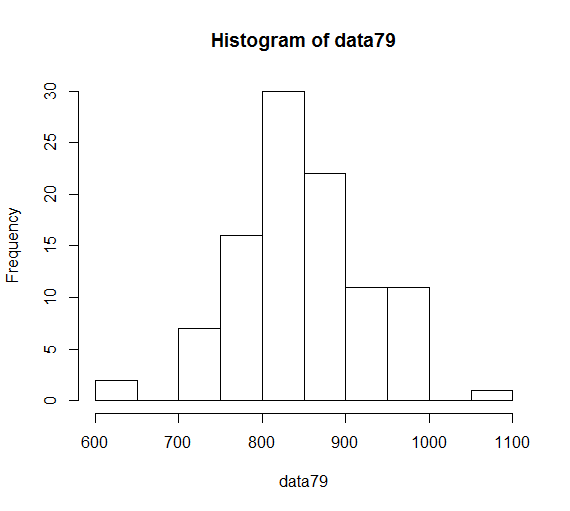
\includegraphics[scale=0.3]{../results/Hist1879.png} }
      \subfigure[1882]
      {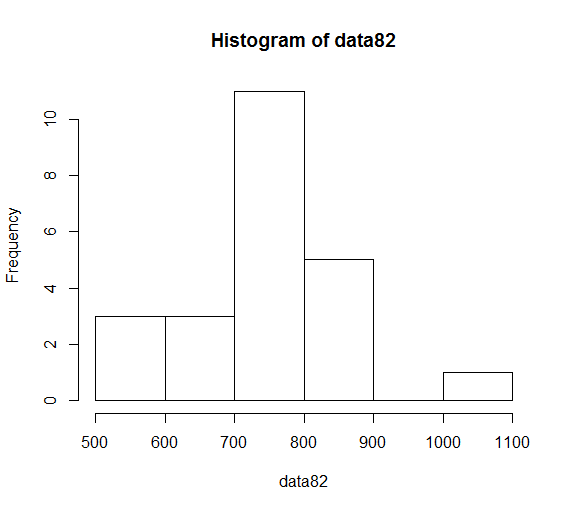
\includegraphics[scale=0.3]{../results/Hist1882.png} }
      \caption{Histograms of the datasets Light1879 and Light1882}
      \label{fig:HistEx2}
    \end{figure}

  \section{Exercise 3}
    Exercise 3 stuff...

  \section{Exercise 4}
    Exercise 4 stuff...

\end{document}